\documentclass[12pt,paper=a4,twosided,cleardoubleage=plain,final]{report}
\usepackage[utf8]{inputenc}

% Hyperreferencing and citations
\usepackage{hyperref}
\hypersetup{
	colorlinks,
	citecolor=blue,
	filecolor=blue,
	linkcolor=blue,
	urlcolor=blue
}

\usepackage{graphicx}
\graphicspath{{images/}}

\usepackage{natbib}

\usepackage{setspace}
\onehalfspacing
% single spacing for table of contents


\usepackage{blindtext}
\usepackage[left=1.5in, right=1in, top=1in, bottom=1in, includefoot, headheight=13.6pt]{geometry}

% To comment multiline text
\newcommand{\comment}[1]{}

\title{
	{Genomic analysis on Sars-Cov-2: \\ A bioinformatics approach}\\
	{\large Anchor University Lagos}\\
	{\vspace{10mm}{
\includegraphics[scale=0.6]{university.png}}}
}
\author{Tekena Solomon}
\date{\today}

\begin{document}
\maketitle

\chapter*{Abstract}
Abstract goes here... % \blindtext


\chapter*{Keywords}
keywords here?

\chapter*{Dedication}
To mum and dad

%\chapter*{Declaration}
%I declare that..

\chapter*{Acknowledgements}
I want to thank...

\tableofcontents
\listoftables
\listoffigures

\chapter{Introduction}
\comment{http://forms.gle/EuVegtneuqaP1HgL7}

\comment{
https://archive.ics.uci.edu/ml/datasets/Heart+Disease
https://www.kaggle.com/datasets/cherngs/heart-disease-cleveland-uci
https://www.hindawi.com/journals/mpe/2021/1792201/
https://www.hindawi.com/journals/cin/2022/2973324/
https://ieeexplore.ieee.org/abstract/document/8740989
https://ieeexplore.ieee.org/abstract/document/6164626
http://citeseerx.ist.psu.edu/viewdoc/download?doi=10.1.1.451.9421&rep=rep1&type=pdf
https://www.researchgate.net/profile/V-V-Ramalingam/publication/325116774_Heart_disease_prediction_using_machine_learning_techniques_A_survey/links/5d48560a299bf1995b68266f/Heart-disease-prediction-using-machine-learning-techniques-A-survey.pdf
}

\section{Background of study}
According to \citefullauthor{2021Cardiovascular}, cardiovascular disease also known as heart disease is one of the leading causes of mortality and morbidity in the world. Over 12 million people die each year as a result of heart disease. Any significant, abnormal condition of the heart or blood vessels is referred to as cardiovascular disease (CVD) (arteries, veins). Coronary heart disease (CHD), stroke, peripheral artery disease, congenital heart disease, endocarditis, and a variety of other disorders are all examples of cardiovascular diseases.

The heart is regarded as one important organ in the body. Any disruption in the heart causes the entire body to be agitated. Sicknesses, including heart disease, are the outcome of daily progressions, and it is notable that heart disease is one of the top five causes of illness worldwide \citep{2021Cardiovascular}. Many cardiovascular problems can be avoided. Over the last few years, the overall prevalence of cardiovascular disease has rapidly increased. Many studies have been conducted in an attempt to determine the most significant factors of cardiovascular disease as well as precisely predict the overall risk. Cardiovascular disease is even shown as a quiet executioner, causing the individual's death without any side effects. Early detection of this disease is critical in making decisions about lifestyle adjustments in high-risk patients to reduce repercussions. In this sense, anticipating heart disease with perfect time and at the correct moment is critical. Machine learning is an important and necessary cycle in defining and discovering useful data and uncovering hidden patterns in massive datasets.

Information mining and Machine Learning technologies are being used in clinical sciences to solve real-world health challenges by forecasting and diagnosing various illnesses.
Machine learning has been shown to be effective in assisting with decision making and forecasting from the massive amount of data given by the medical industry. This project hopes to predict the risk of heart disease by analysing patient data that characterizes whether or not they will have cardiovascular disease using machine learning algorithms. Even though heart disease can emerge in many forms, there is a standard set of risk variables that influence whether or not someone will eventually be at risk of heart disease. 


\section{Problem statement}
The most challenging task in coronary sickness is recognizing it. There are tools available that can predict heart disease, however they may be expensive or ineffective in determining the risk of coronary sickness in individuals. Early detection of heart diseases can reduce death rates and general discomfort. However, screening patients on a regular basis in all instances is absurd, and consulting an expert for 24 hours by a patient is not feasible because it demands more understanding, time, and skill. Because we have so much information in this day and age, we can use various machine learning algorithms to search for hidden patterns in medical data. These hidden patterns can be used for health diagnosis of possible risk of heart disease.

\section{Significance of study}
The Heart disease machine learning software will predict the likelihood of patients getting heart disease. It enables immense data, for instance, relationships between clinical variables connected with heart disease and patterns, to be laid out. Also, the software will provide an inference based off the medical data inputted by its users. The proposed system will help users, researchers and medical practitioners to know if an individual is likely to have heart disease based off their medical data.

\comment{Chapter organization}
\section{Motivation}
The key contribution that this work makes is the presentation of a heart disease prediction system, which can assess the likelihood of an individual developing heart disease. In addition to that, the purpose of this research is to determining whether or not a patient is at risk of having heart disease and provide some expert knowledge based on the user's medical data. This work is genuine since it does a relative report and analysis using four classification algorithms, specifically Decision Tree, Naive Bayes, Logistic regression and K-nearest neighbours, at various levels of assessment. Although these are commonly used machine learning methods, heart disease prediction is a critical task requiring the highest possible precision. As a result, the four algorithms are evaluated to determine the best in predicting heart disease. Some of the reviewed studies includes
\citefullauthor{waghulde2014genetic} research on heart disease which led them to collect information about multi-facet neutral networks and back spread learning calculations for network preparation. \cite{srinivas2010applications} suggested that data mining strategies be used to predict cardiovascular failure. He focused on arrangement calculations, such as Decision tree and Naive Bayes, to tell if a stroke infection was present. \cite{pattekari2012prediction} used the Naive Bayesian Classification procedure to help people make decisions in the coronary illness expectation framework. In the end, the problem with all of these projects is that they did not design a system that allows users easy access to use the models. Also, the proposed systems were limited such that they did not provide a way for users to have more knowledge about the inputted health data.

\section{Aim and objectives}
The aim of this project is to develop a heart disease prediction system using machine learning techniques that effectively serves both patients and health care centres, particularly in medical institutions, and to build a submodule that provides inference (expert knowledge) based on user's medical data and prediction output. 

The objectives of the study are to:
\begin{enumerate}[label=(\alph*)]
	\item  design  of a heart disease prediction model for hospitals and medical centres
	\item an inference engine that provides inference based on the prediction output and information provided by the patient
\end{enumerate}

\section{Methodology}
The methods used in the study include creating machine learning models using classification algorithms to predict the risk of heart disease. These models are trained, tested and saved for in in a web application. The web app provides an interface for users to interact with the machine learning model. After prediction by the model, an inference engine produces expert knowledge about the health data from rules encoded in a knowledge base. More detailed information about the methodology will be discussed in \hyperref[chap:3]{Chapter 3}

\comment{The scope of study}
\section{Scope of study}
The primary audience for this study is researchers, hospitals and medical clinics. The implementation will begin with the health care centre that is located within Anchor University, and it is possible that it may be expanded to include additional medical institutions located within Nigeria.


\section{Limitations of study}
There are few drawbacks to be aware of. These include:

At the first release, the heart disease prediction may not have all the features desired by medical practitioners.

Due to time constraints, the first release may not have all intended functionalities like a well formed knowledge base, but would be improved upon in the nearest future.


\chapter{Literature Review}
\section{Introduction}
In this chapter, the review of literature relevant to the study area of the heart disease prediction using machine learning techniques is carried out and one of the major focuses is to explain the history and empirical basics of this study.

\section{Review of related literature}
A. Taneja (2013), applied data mining and AI calculations to be specific, Decision Tree (J48 calculation), Artificial Neural Networks (ANN), Naive Bayes, and for heart illness forecast. A dataset of 7339 occasions with 15 elements has been selected from PGI Chandigarh. WEKA 3.6.4 instrument was utilized for the test. For model preparation and testing 10-Fold, Cross-Validation strategies are utilized arbitrarily. Best First Search strategy was utilized to select the most ideal attributes from the available 15 ascribes and among them just 8 attributes have been chosen. Each experiment was finished in two distinct situations, the initial one containing each of the 15 attributes and the second case just 8 selected attributes.

Celia et al. 2000 research that characteristic determination can be performed preceding hereditary programming to tracking down an elevated degree of reasonable information. Following this review, Hongmei Yan fostered a multiplayer perceptron-based choice help system to help the determination of coronary heart disease (Hongmei Yan 2006). This framework is very much designed as an info layer of the framework with 40 information factors and is classified into four groups and afterward encoded utilizing the proposed coding plan.

R. Setthukkarasi (2016) has fostered another neutral fluffy strategy to analyze current realities of the illness in patients reports. The summed-up database is designed for decision-production from a diminished arrangement of qualities, which is the result of the hereditary calculation. Four layered fluffy neutral networks are utilized for effective displaying and surmising with time reliance under vulnerability. Chaitrali Dangare (2001) has carried out a framework for foreseeing heart disease and has applied three data mining order procedures: Decision trees, Naive Bayes and Neural Networks. The outcomes show that neutral networks are better than decision trees and Naive Bayes.

Nilakshi P. Waghulde and Nilima P. Patil (2020) performed heart disease informational collection regarding multi-facet neutral networks related to back spread learning calculations for network preparing. A weighting calculation is utilized to improve neutral network initialization. This study shows the consequences of the Genetic Neural Network for heart illness expectation, utilizing an ideal neutral network design that predicts whether a patient is experiencing coronary illness, further developing accuracy by 98%

Sudha et al (2020). concentrated on arrangement calculations, for example, Decision tree and Naive Bayes to distinguish stroke infection. Classification methods, for example, decision trees, Bayesian classifiers, and backpropagation neutral networks were utilized in this review. Records with irrelevant information were erased from the information distribution center before the mining system occurred.

K. Srinivas (2017) proposed the use of data mining strategies to the forecast of cardiovascular failure. The creators concentrated on grouping-based data mining strategies, for example, rule based, choice trees, Naive Bayes, and counterfeit neutral networks for a tremendous measure of clinical data. The Tanagra information mining apparatus was utilized to inspect data investigation, machine learning, and statistical learning algorithms. They utilized a preparation informational collection of 3000 examples with 14 distinct properties. Cases of the informational index address the consequences of different test types to foresee the exactness of heart disease.

Carlos Ordonez (2001) studied on the prediction of heart disease with the assistance of affiliation rules. They utilized a straightforward planning calculation. This algorithm regards attributes as numeric. It is utilized to change over clinical records into exchange designs. Improved calculations are utilized to minify confined affiliation rules. The mapping table is ready and the characteristic worth is planned to the item. Decision trees are utilized for data mining since they naturally partition numeric qualities. Split points chosen in the choice tree are seldom utilized. Grouping is utilized to acquire a general comprehension of the data

P. Chandra and M. Jabbar (2016) utilized the element subset determination to make class affiliation rules to detect heart disease. Affiliation rules decide the connection between characteristic qualities and grouping to predict classes in a patient data index. Functional selection, like a hereditary pursuit, decides the qualities that assist with foreseeing heart disease. Usha Rani (2016) proposed a framework for anticipating heart disease with a blend of feedforward and backpropagation algorithms with the assistance of artificial neural networks. Tests are performed considering single and multi-facet neural network models. Parallel processing is carried out to speed up the growing experience in every neuron of all hidden result layers.


Shadab Adam Pattekari and Asma Parveen (2018) utilized the Naive Bayesian Classification procedure to foster choice support in the coronary illness expectation framework. The framework tracks down hidden information from past coronary illness datasets. This is the best model for anticipating coronary illness. The model can answer complex questions and has its own solidarity concerning simplicity of model understanding, admittance to more precision  and information.

Huiyan Wang (2008) has sought after a specialty in this sward by proposing a mechanized symptomatic model to advance normalization and promotion of conventional Chinese medication (TCM) finding. The framework fills in as follows. First, the incidental effects are picked by acquiring the Bayesian association structure from a data set of cases that coordinate normal information speculation. In the design, the Markov blanket of the objective variable is chosen as the side effect set. Second, the planning connections between side effect sets and indicative results relies on naive Bayesian classifiers.

The next venture in the field was by Huang Jianyong (2004). This review aims to tackle the issue of multiclass grouping utilizing parallel classifiers. The paired characterization tree configuration is done so that the class group is separated into two distinct subsections from one hub. The hub takes on the class module strategy to further develop the binary characterization capacity. Partitioning is planned as an improvement issue, and, hereditary calculations are proposed to tackle advancement issues. Heart mumbles were a significant issue in pediatric cardiovascular illness, and this gathering  had a high occurrence of cardiovascular commotion (77\% - 95\% as reported), bringing about little blockage because of intrinsic coronary illness. Sanjay (Sanjay 2005) has fostered a dependable test gadget to analyze mumbles in pediatrics.


Salam Ismaeel et al, (2021) the fundamental target of this review is to supplant the expensive clinical check-up by an advance warning framework for patients that are probably going to experience the ill effects of heart disease. The proposed approach utilizes outrageous machine learning algorithm to show the different qualities of the dataset which is ongoing information gathered by the sever land clinical establishment containing 300 examples. The two machine learning technique Utmost Machine Learning and ANN were utilized for the investigation among which utmost Machine Learning shows the most highest precision of 87\%. The Utmost machine learning algorithm has five (0-4) results and utilizing this model, the analysis of new patient should be possible utilizing the past information.

Monika Gandhi et al (2015). The fundamental aim in this study is the mechanization of such framework for diagnosing heart disease by thinking about earlier data and information. It plans to give details of different strategies of information deliberation by utilizing data mining techniques, including their benefits and negative marks.

M.Akhil jabbar et al. (2013) proposed an approach which consolidates KNN with a Genetic model. The wellspring of the dataset is UCI AI repository including 5 attributes and 14 examples. The proposed model was not effective for essential growth and breast cancer because of immaterial and excess elements present in the dataset. The outcomes uncover the get-over rate for hereditary calculation is 60\% KNN, the review shows expansion in precision for expectation of coronary illness.

Deepika (2011) concentrated on Pruning-Classification Association Rule (PCAR) to remove affiliation rules. PCAR has given an analysis of the Apriori algorithm. PCAR covers a bunch of least frequency, which eliminate unpredictable things from a bunch of things. It then, at that point, sorts the arrangement of things in light of the recurrence of the arrangement of things and tracks down a successive arrangement of items. Ordonez utilizes affiliation rules in data mining to get better coronary illness prediction results. The authors concentrated on the limitation of affiliation rules that mined the whole data collection without check of autonomous samples. We presented calculations that changed the inquiry limitations to decrease the quantity of affiliations runs and approved them utilizing train and test approaches. They have concentrated on two corresponding tasks which are anticipating the absence and foreseeing the presence of coronary illness.

K. Srinivas (2019) proposed the use of data mining strategies to the prediction of cardiovascular failure. The authors concentrated on grouping-based data mining strategies, for example, decision trees, rule-based, Naive Bayes, and artificial neural networks for a tremendous measure of clinical information. The Tanagra data mining apparatus was utilized to look at data investigation, machine learning, and measurable learning algorithms. They utilized a preparation informational collection of 3000 cases with 14 distinct properties. Examples of the informational collection address the results of different test types to anticipate the precision of coronary illness.

C. Sowmiya and P.Sumitra (2020) acknowledge that It is crucial to have a system that can practically perceive the pervasiveness of coronary illness in countless tests immediately. The authors evaluated the ability of nine grouping strategies for the prediction of coronary illness. Specifically, decision tree, naive Bayesian neural network, SVM.ANN, KNN. The proposed algorithm of Apriori estimation and SVM (support vector machine) in coronary illness prediction. Utilizing clinical profiles, for example, blood pressure, fasting blood sugar, and chest pain type. It can foresee the likelihood of patients getting a coronary illness. Because of this, medical society checks out distinguishing and preventing coronary illness. The investigation it has exhibited that classification-based procedures contribute to high viability and acquire high exactness accuracy compared to the previous methods.

Marjia et al (2018), created heart disease prediction utilizing KStar, SMO, j48, Bayes Net and Multilayer perception utilizing WEKA system. In light of execution from various component SMO and Bayes Net accomplish ideal execution than KStar, Multilayer perception and J48 strategies utilizing kfold cross approval. The exactness of these algorithms is additionally not agreeable. The precision of the outcomes is therefore improved to empower a superior indicative decision.

M.Raihan et.al (2019) has fostered a straightforward way of forecasting the probability of ISD utilizing a smartphone. The use of clinical data gathered from patients conceded with IHD has developed Android-based model applications. Clinical data from 787 patients was examined with risk factors, for example, hypertension, diabetes, raised cholesterol, smoking, obesity, depression, and current clinical side effects that might show the hidden unrecognized  IHDs. Data were separated and a score was produced utilizing data mining digging innovation Risks for IHD are reviewed as low, medium, and strong. The authors observed that a significant relationship among low-and medium-and high-grade cardiovascular occasions was noticed for patients whose data were gathered to deliver the evaluations, individually; p=0.0001 and 0.0001. They gave a basic approach to recognizing the risk of IHD and are inclined to cardiology to keep away from sudden deaths. As of now, there are a couple of constraints on the open resources that make them unused by the population.

Sarath Babu et al. (2016) have proposed that clinical data mining will investigate the mystery patterns of clinical informational indexes with extraordinary potential. These patterns might be utilized to diagnose clinically. The data should be gotten in an organized way. From the medical services profiles, the patient can be anticipated by 14 attributes. MAFIA algorithms and decision tree order, utilizing data mining innovation to analyze heart diseases can accomplish as much accuracy as possible while diagnosing a heart condition. These medical industries could offer better findings and treatment of the patient to accomplish a decent nature of services. The primary benefits pointed out in the exploration are: early recognition of heart disease and its diagnosis accurately on time and providing treatment with affordable expense.

According to Senthil Kumar et.al (2019), Machine learning has been indicated to be viable in serving with simple choices and forecasts from the tremendous measures of data delivered by the medical services industry. Machine learning methods are being used in ongoing improvements in various regions of the Internet of Things (IoT). Different investigations give just a brief look into predicting heart disease with machine learning procedures. Authors proposed a clever methodology that targets tracking down huge elements by applying machine learning procedures bringing about working on the precision in the estimate of cardiovascular sickness. The prediction model is given different mixes blends of features and a couple of known grouping procedures. We produce an improved performance level with an accuracy level of 88.7\% through the prediction model for coronary illness with the hybrid irregular forest with a linear model (HRFLM).

M.A.Zabbar and Shirina Samree (2019) said that heart disease is an overall driving reason for death. According to the authors, heart diagnosis is a dreary undertaking, and a savvy dynamic emotionally supportive system for the prediction of sicknesses is required. Strategies for data mining are additionally used to evaluate the patient's typical heart condition. Hidden Naive Bayes is a kind of data mining that loosens up the regular autonomy of the Naïve Bayes. The model proposed noticed that the Hidden Naïve Bayes can be applied to the characterization of heart sicknesses

According to Ed-Daoudy (2019), early identification of heart sicknesses and constant checking can decrease the mortality rate. The remarkable development of data from different sources, for example, wearable sensor gadgets utilized in Internet of Things health monitoring, real-time framework, and others have been producing a colossal measure of data consistently. The combination of streaming huge data storage and machine learning is a cutting-edge innovation that can have a critical effect in the medical care field particularly early detection of coronary illness. This alteration can be even more astounding and more reasonable. A continuous heart disease prediction framework has been proposed in light of Apache Spark. The framework comprises two principal sub-parts, to be specific streaming processing and visualization.

Amin Ul Haq et.al (2018) have concocted a Hybrid Intelligent System Framework for the Prediction of Heart Diseases. The authors declared that noninvasive-based techniques, for example, machine learning are dependable and proficient. A Machine-learning-based diagnosis framework for heart disease prediction by utilizing a heart disease prediction dataset was created utilizing seven famous machine learning algorithms, three feature selection algorithms, the cross-approval technique, and seven classifiers execution assessment measurements like grouping exactness, explicitness, responsiveness, Matthews' relationship coefficient, and execution time. The proposed framework can undoubtedly distinguish and arrange individuals with heart disease from healthy people. Furthermore, receiver optimistic curves and regions under the bends for every classifier were figured. The authors validated the performance of the proposed framework on full elements and a diminished arrangement of elements. The component decrease affects classifier execution to the extent that precision and execution time of classifiers.

Md. Shahriare Satu et.al (2021) present that heart disease is one of the main infections that cause huge loss of lives from one side of the country to the other. A couple of astonishing ways of figuring out basic factors of heart contaminations have been seen by the creators. Values of the different extent of individual attributes in these data are determined to figure out significant components of this affliction. Then, semi-regulated learning algorithms, for example, Collective Wrapper, Filtered Collective, and Another Semi-Supervised Idea are utilized to investigate heart disease data. Assessments of these classifiers like exactness, f-measure, region under ROC still hanging out there to legitimize individual classifiers and show the best semi-managed learning algorithm. This calculation is researched enormous and unessential components of coronary illness by wiping out credits in a consistent movement successively and noticing the results of request. Exploratory results on two veritable data demonstrate the reasonability and productivity of the analysis.

R. Sharmila et al, (2018) proposed a non-linear heart disease prediction order algorithm. Large data instruments like the Hadoop Distributed File System (HDFS) are proposed for heart infection prediction with advanced trait depiction. This proposition examined the usage of various systems data mining for heart sickness prediction. This proposes to use HDFS to store a lot of data in various hubs and run the forecast algorithm simultaneously involving SVM in more than one hub. SVM is utilized in parallel, providing preferred time over successive SVM computing.


\chapter{Methodology}
\comment{https://www.youtube.com/watch?v=sgQAhG5Q7iY}
\noindent
The proposed system is divided into three major components shown in \figurename~\ref{fig:sytem-overview} which includes the web client, web server and machine learning models. The web interface get the user health data and sends it to the web server for processing. The web server passes the data to the trained model and returns the binary output which the user sees.

\begin{figure}[htb]
	\centering
	\makebox[0cm]{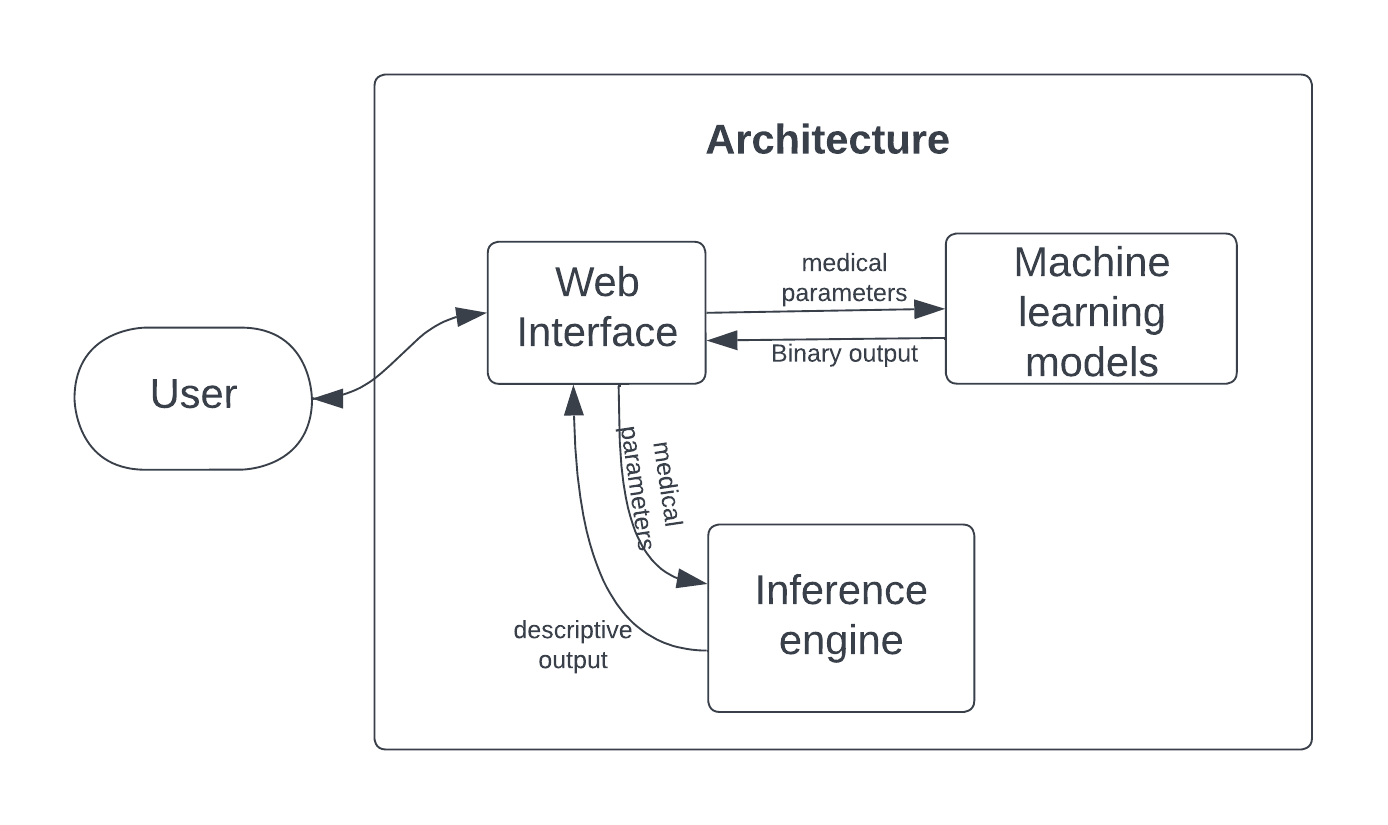
\includegraphics[scale=0.3]{system-overview.png}}
	\caption{System overview}
	\label{fig:sytem-overview}
\end{figure}


\section{Machine learning workflow}
\figurename~\ref{fig:ml-workflow} shows the workflow of for creating the machine learning model.

\begin{figure}[htb]
	\centering
	\makebox[0cm]{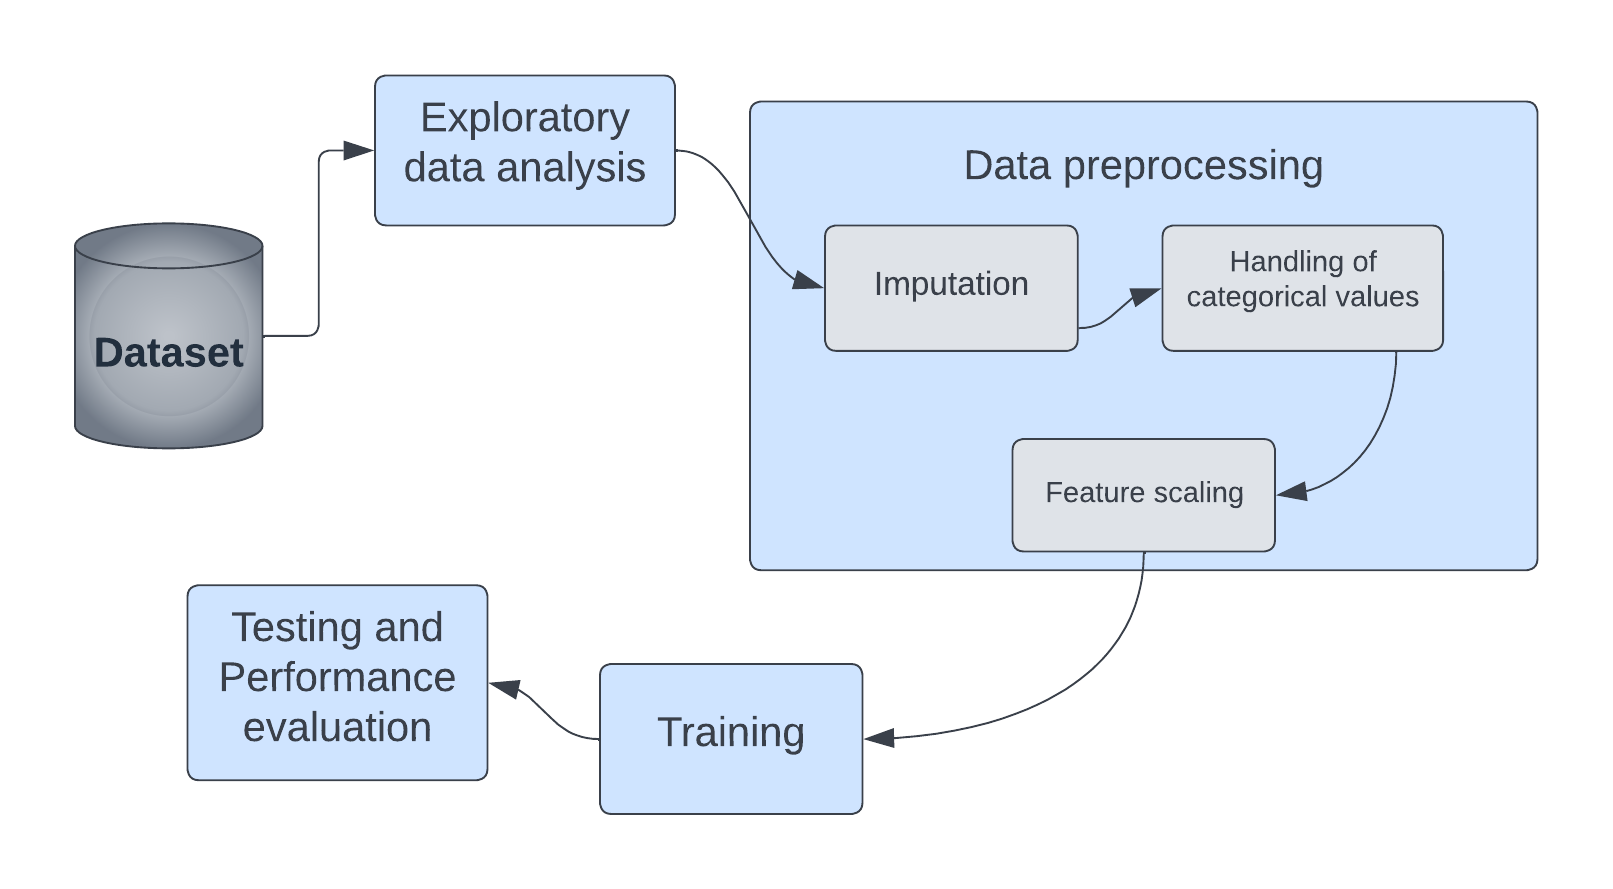
\includegraphics[scale=0.3]{ml-workflow.png}}
	\caption{Machine learning workflow}
	\label{fig:ml-workflow}
\end{figure}

\subsection{Dataset}
An estimated 17.9 million people die each year as a result of cardiovascular diseases (CVDs), making up 31\% of all deaths worldwide. Heart attacks and strokes are the cause of mortality for three-quarters of people under the age of 70 who die from CVD. Several CVDs can lead to heart failure, and this dataset comprises 11 variables that can be used to gauge the likelihood of heart failure \citep{world-health-organization-2019}.

An early diagnosis and management strategy can be of significant use to people with coronary heart disease or those at high risk of developing the illness because of the existence of risk factors such as hypertension, diabetes, and hyperlipidaemia.

\subsubsection{Features}
These features represent the different columns in the dataset
\begin{enumerate}[label=(\alph*)]
	\item{\textbf{Age:} age of the patient [years]}
	\item{\textbf{Sex:} sex of the patient [M: Male, F: Female]}
	\item{\textbf{ChestPainType:} chest pain type [TA: Typical Angina, ATA: Atypical Angina, NAP: Non-Anginal Pain, ASY: Asymptomatic]}
	\item{\textbf{RestingBP:} resting blood pressure [mm Hg]}
	\item{\textbf{Cholesterol:} serum cholesterol [mm/dl]}
	\item{\textbf{FastingBS:} fasting blood sugar [1: if FastingBS $>$ 120 mg/dl, 0: otherwise]}
	\item{\textbf{RestingECG:} resting electrocardiogram results [Normal: Normal, ST: having ST-T wave abnormality (T wave inversions and/or ST elevation or depression of > 0.05 mV), LVH: showing probable or definite left ventricular hypertrophy by Estes' criteria]}
	\item{\textbf{MaxHR:} maximum heart rate achieved [Numeric value between 60 and 202]}
	\item{\textbf{ExerciseAngina:} exercise-induced angina [Y: Yes, N: No]}
	\item{\textbf{Oldpeak:} oldpeak = ST [Numeric value measured in depression]}
	\item{\textbf{ST\textunderscore Slope:} the slope of the peak exercise ST segment [Up: upsloping, Flat: flat, Down: downsloping]}
	\item{\textbf{HeartDisease}:output class [1: heart disease, 0: Normal]}
\end{enumerate}

\subsubsection{Target variable}
In the context of machine learning, the term "target variable" refers to the variable that either is or should be the output. If you are classifying the data, for instance, it could be a binary 0 or 1, but if you are running a regression, it could be a continuous variable. In the field of statistics, this concept is also known as the response variable.

In the context of this research, the variable HeartDisease serves as our target variable. We are interested in identifying whether or not somebody is likely to get heart disease based on the input parameters such as gender, age, and the results of numerous tests.

\subsection{Exploratory data analysis}
Exploratory data analysis, (EDA) is the important process of looking at data for the first time to find patterns, find outliers, test hypotheses, and check assumptions with the help of summary statistics and graphical representations. This is done to make sure that the data are correct and can be reliable. 

\subsubsection{Importance of exploratory data analysis}
There are several reasons for performing EDA which includes; understanding the dataset helps clean up the dataset; gives a clear idea of the features and how they fit together; gives guidelines for what variables are important and what variables can be left out or taken away; handling of missing values or human error; help get the most information out of the dataset.


\subsection{Data preprocessing}
Data preprocessing is required for accurate data representation and machine learning classifiers, for proper training and evaluation. For the dataset to be used effectively by the classifiers, preprocessing methods such imputation, feature scaling and handling of categorical variable have been applied.

\subsubsection{Imputation}
Imputation is a straightforward operation that involves replacing the values in our dataset that are absent (null). We can accomplish this by implementing our own specialized function, or we can simply perform imputation by making use of sklearn's built-in SimpleImputer class. Both of these options are available to use. For example:
\begin{lstlisting}[language=Python, numbers=none, label={lst:simple-imputer}]
	from sklearn.impute import SimpleImputer
	
	imputer = SimpleImputer(missing_values=np.nan, strategy='mean')
	imputer = imputer.fit(df[['Weight']])
	df['Weight'] = imputer.transform(df[['Weight']])
\end{lstlisting}

\subsubsection{Feature scaling}

Feature scaling is a method for uniformly reducing the values of each independent feature in our dataset. Algorithms can be calculated much more quickly with the aid of feature scaling making it a significant step in the preprocessing of data. The machine learning models would give larger weights to higher values and lower weights to lower values if we hadn't scaled the features. Additionally, training the machine learning model will take a longer time without scaling. The standard scalar is a feature scaling method that guarantees that they all have the same mean and variance. Although there were no features with missing values in the dataset, it is a recommended practice to check for and remove data units with missing values. These data preprocessing methods were all applied in this study.

\subsubsection{Handling of categorical variables}
Categorical variables/features are any feature type can be classified into two major types:
\begin{itemize}
	\item Nominal
	\item Ordinal
\end{itemize}
Nominal variables are those that have two or more categories that are not in any particular order. For example, gender can be thought of as a nominal variable if it is split into two groups, male and female. On the other hand, ordinal variables have "levels" or categories that are in a certain order. For example, an ordinal categorical variable can be a feature with three levels: low, medium, and high. Order is important.

This is a binary classification problem, and although the target is not skewed, we apply the best metric for it, which is the area under the ROC curve (AUC). Although precision and recall are also options, AUC combines precision and recall. As a result, we will use AUC to assess the model that we create using this dataset.

Since text data cannot be understood by computers, we must transform these categories to numbers. This may be done easily by using:

\begin{itemize}
	\item{Label Encoding: using sklearn's LabelEncoder class}
	\begin{lstlisting}[language=Python, caption=Label Encoder, numbers=none]
	from sklearn.preprocessing import LabelEncoder\end{lstlisting}
	\item{One Hot Encoding: using sklearn's OneHotEncoder class.}
	\begin{lstlisting}[language=Python, caption=Get dummies, numbers=none]
	from sklearn.preprocessing import OneHotEncoder\end{lstlisting}
\end{itemize}
But we must know when to apply which kind of label encoding: \\
\\
\noindent
\textbf{One-Hot Encoding is the best use for non-tree based Machine Learning Algorithms.}
\begin{itemize}
	\item The advantage of One-Hot-Encoding is that the result is binary rather than ordinal and that everything is in an orthogonal vector space.
	\item The negative is that with large cardinality, the feature space can quickly explode and you are forced to deal with the curse of dimensionality. In these circumstances, I usually use one-hot encoding followed by PCA to reduce dimensionality. Other encoding strategies rarely outperform the prudent combination of one-hot plus PCA, in my opinion. Because PCA detects linear overlap, it will naturally group comparable features together.
\end{itemize}

\noindent
\textbf{For tree based algorithms, label encoding is the best way to go.}

\begin{itemize}
	\item{LabelEncoder can convert [dog,cat,dog,mouse,cat] to [1,2,1,3,2], however the required ordinality means that cat is the average of dog and mouse. There are still algorithms that operate well with categorical variables, such as decision trees and random forests, and LabelEncoder can be used to store values with minimal disk space.}
\end{itemize}

\comment{

\subsubsection{Cross validation \& Hyperparameter optimisation}
In machine learning, choosing the best hyperparameters for a learning algorithm is called hyperparameter optimization or tuning. It is possible to regulate the learning process by altering a parameter's value, which is known as a hyperparameter. It's a different case when it comes to learning other parameters (usually node weights).
1
The same machine learning model may need various constraints, weights, or rates of learning to generalize to diverse patterns of input data. These parameters, also known as hyperparameters, must be fine-tuned to ensure that the model is able to tackle the machine learning problem to its full potential. To minimize a predetermined loss function on provided independent data, a hyperparameter optimization model is constructed by finding a pair of hyperparameters that minimizes the loss function. The loss associated with a tuple of hyperparameters is returned by the objective function. As a generalization test, cross-validation is commonly utilized.
}



\subsubsection{Cross validation}
In cross-validation, training data is split into a few parts. Some of these parts are used to train the model, and the rest are used to test it.

The best cross-validation method to use will depend on the dataset you are working with, and it may or may not be applicable to other datasets. There are a few cross-validation techniques, though, that are the most well-known and frequently employed. These consist of:

\begin{enumerate}[label=(\alph*)]
	\item K-fold cross-validation.
	\item Stratified k-fold cross-validation
\end{enumerate}

You shouldn't use random k-fold cross-validation if you have a skewed dataset for binary classification with 90\% positive samples and only 10\% negative samples. If you use simple k-fold cross-validation on a set of data like this, you might end up with folds that have no positive samples at all. We like to use stratified k-fold cross-validation in these situations. The number of labels in each fold stays the same with stratified k-fold cross-validation. So, you will have the same 90\% positive and 10\% negative samples in each fold. So, no matter what metric you use to measure, the results will be the same for all folds. So in the case, we would be using stratified k-fold cross-validation technique.

\comment{
\subsection{Training the models}
The following machine learning algorithms will be used for building the classification model.


}

\subsection{Performance evaluation}
When it comes to classification problems, the following measures are most frequently used:

\begin{enumerate}[label=(\alph*)]
	\item{Accuracy}
	\item{Precision (P)}
	\item{Recall (R)}
	\item{F1 score (F1)}
	\item{Area under the ROC (Receiver Operating Characteristic) curve or simply AUC (AUC)
		\begin{itemize}
			\item {When you have a dataset with skewed binary targets, another measure that is frequently employed is the area under the ROC curve calculation. The Area Under ROC Curve, Area Under Curve, or plain AUC are all names for this measure. The area under the ROC curve can be calculated in a variety of methods.}
			\item{AUC is a metric that is frequently used in machine learning for skewed binary classification tasks.}
		\end{itemize}
	}
\end{enumerate}

\section{Web interface}
The web interface consists of the web server and client components that provides a way for users to interact with the machine learning algorithms.

\begin{figure}[htb]
\centering
\makebox[0cm]{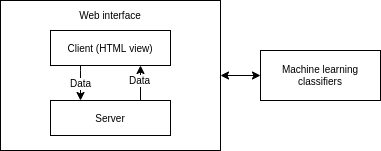
\includegraphics[scale=0.8]{web-interface.png}}
\caption{Web interface}
\label{fig:web-interface}
\end{figure}

A web server is software and hardware that responds to client requests sent over the World Wide Web using the HTTP (Hypertext Transfer Protocol) and other protocols. A web server's primary responsibility is to show website content by storing, processing, and sending webpages to users.

The web server is built in python with the python \href{https://flask.palletsprojects.com/en/2.1.x/}{flask} web framework using \href{https://jinja.palletsprojects.com/en/3.1.x/}{jinja} as a templating engine for the client interface. The server extracts the input data from a form the user submits via an API endpoint and validates the data so there is no invalid input. The implementations of the server will be discussed in \autoref{chap:4}.

\begin{figure}[htb]
	\centering
	\makebox[0cm]{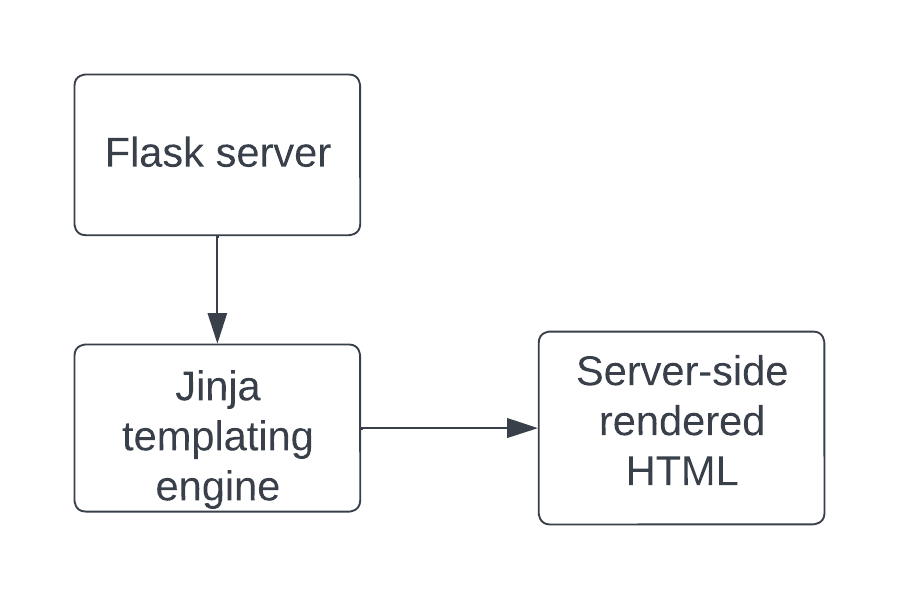
\includegraphics[scale=0.3]{server.png}}
	\caption{Server}
	\label{fig:server}
\end{figure}

\subsection{Flask}
Flask is a lightweight Python web framework. It is called a micro-framework because you don't need any special tools or libraries to use it. It doesn't have a database abstraction layer, a form validation layer, or any other part where existing components are already provided by third-party libraries.
\subsection{Jinja}
Jinja is a Python programming language web template engine. Armin Ronacher developed it, and it is released under the BSD License. Jinja is comparable to the Django template engine, but it supports Python-like expressions and ensures that templates are evaluated in a sandbox.

\section{Inference engine}
In order to provide a response, an inference engine analyzes the facts included in the knowledge base and makes interpretations based on those evaluations. The inference engine in this study consists of a knowledge base and a parser. The knowledge base contains the expert knowledge encoded as rules in a yaml file. These encoded rules are then parsed by a parser which then generates inference based on the medical data.

\begin{figure}[htb]
	\centering
	\makebox[0cm]{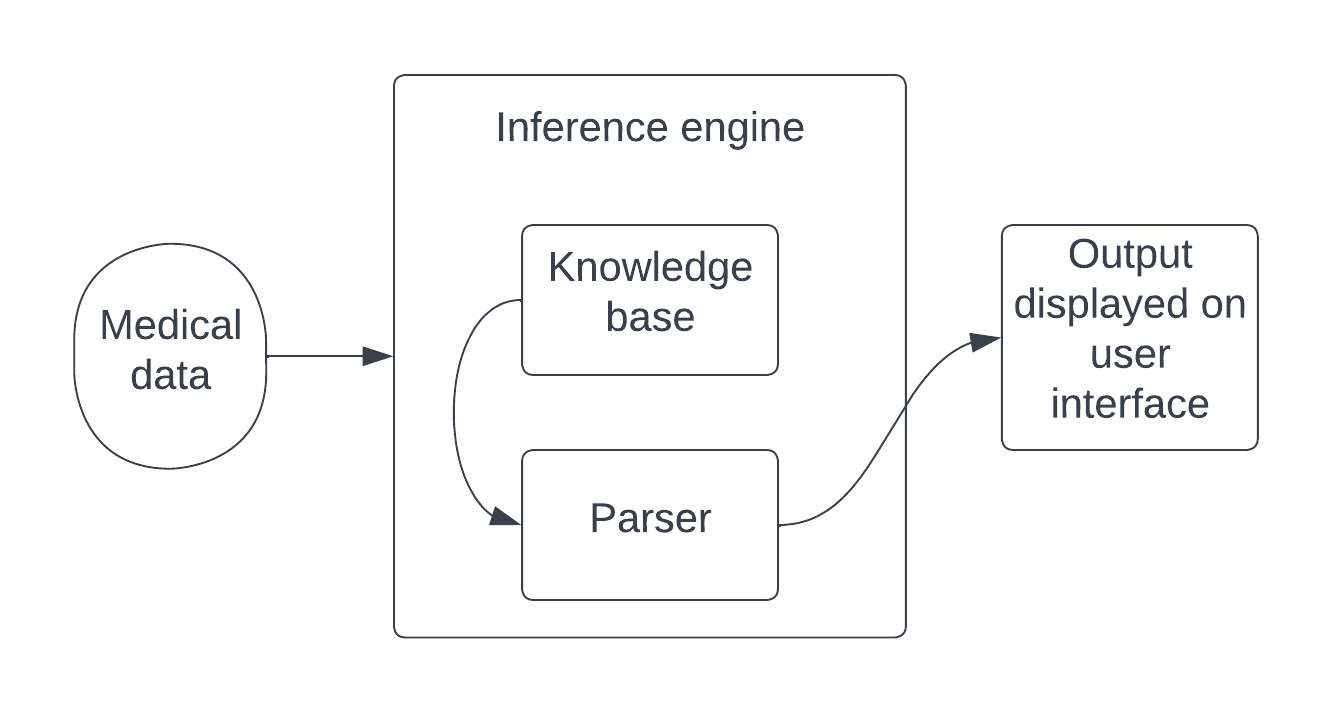
\includegraphics[scale=0.3]{inference-engine.png}}
	\caption{Inference engine}
	\label{fig:inference-engine}
\end{figure}


\chapter{Results}

\section{Machine learning module}
\subsection{Dataset source}
The dataset used is gotten from \href{https://www.kaggle.com/datasets/fedesoriano/heart-failure-prediction}{kaggle} and was made by putting together different datasets that were already out there but had never been put together before. In this dataset, 5 heart datasets are put together based on 11 common features. This makes it the largest dataset for heart disease research that has been made available so far. The five datasets that were used to put it together are:
\begin{enumerate}[label=(\alph*)]
	\item Cleveland: 303 observations
	\item Hungarian: 294 observations
	\item Switzerland: 123 observations
	\item Long Beach VA: 200 observations
	\item Stalog (Heart) Data Set: 270 observations
\end{enumerate}

\comment{The classification process was carried out with the use of k-nn, naive bayes, decision tree, and logistic regression algorithms.}

\subsection{Exploratory data analysis}

\subsubsection{Correlation chart}
A correlation matrix is nothing more than a table that displays the correlation coefficients for various variables. The matrix illustrates the relationship between all possible pairings of values in a table. It is a strong tool for summarizing a large dataset as well as identifying and visualizing trends in the data.

\begin{lstlisting}[language=Python, caption={Correlation chart}]
	pd.options.display.float_format = "{:,.3f}".format
	plt.figure(figsize=(10,8))
	sns.set_context('notebook',font_scale = 1.15)
	sns.heatmap(df.corr(),annot=True, linewidths=1)
	plt.savefig("corr.png")
	plt.show()
\end{lstlisting}
\begin{figure}[htb]
	\centering
	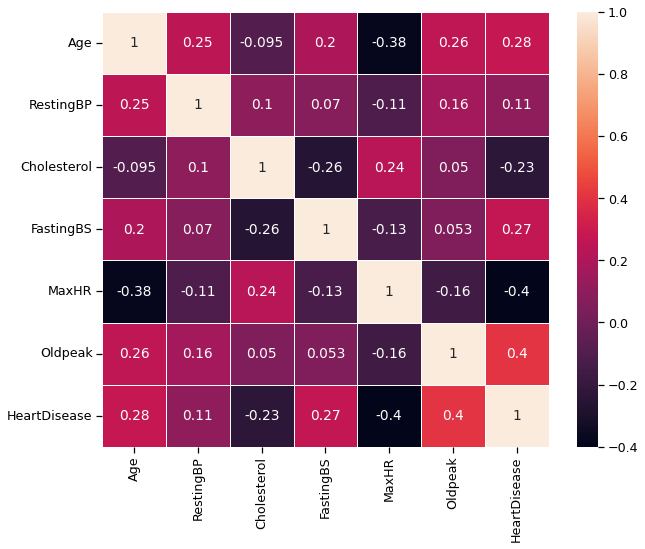
\includegraphics[scale=0.65]{correlation-chart.png}
	\caption{Correlation chart}
	\label{fig:correlation-chart}
\end{figure}
From the correlation chart \figurename~\ref{fig:correlation-chart} we can see that:
\begin{enumerate}[label=(\roman*)]
	\item{Oldpeak is highly positively correlated to the target variable.}
	\item{MaxHR is highly negatively correlated toe the target variable.}
	\item{RestingBP has the lowest correlation compared to other attributes}
\end{enumerate}
\subsubsection{Plotting numerical values}
In Listing~\ref{lst:plot-numerical} I plotted age and fasting blood sugar count with the target column.
\begin{lstlisting}[language=Python, caption={Plotting select numerical features with target column}, label={lst:plot-numerical}]
	cols_to_plot = ["Age", "FastingBS"]
	for i in cols_to_plot:
		plt.figure(figsize=(14,5))
		sns.countplot(x=df[i], data=df, hue='HeartDisease')
		plt.legend(['Normal', 'Heart Disease'])
		plt.title(i)
		plt.tight_layout()
\end{lstlisting}
\comment{
\begin{figure}[htb]
	\centering
	\begin{floatrow}
		\ffigbox[\FBwidth]{\caption{Ages chart}\label{}}{
			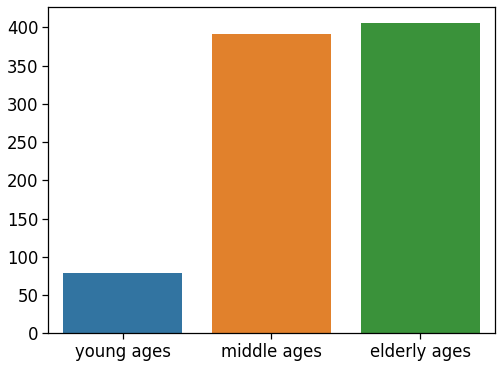
\includegraphics[scale=0.4]{ages-chart.png}}
		\ffigbox[\FBwidth]{\caption{FastingBS chart}\label{}}{
			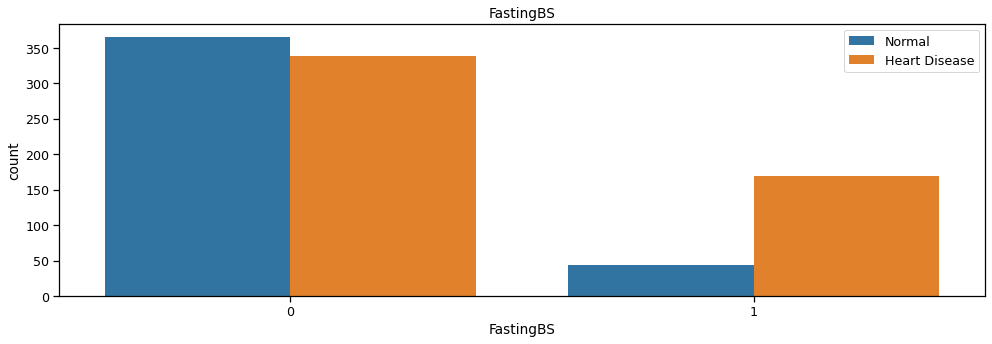
\includegraphics[width=3in, height=3in]{fasting-bs-chart.png}}
	\end{floatrow}
\end{figure}
}

\begin{figure}[htb]
	\centering
	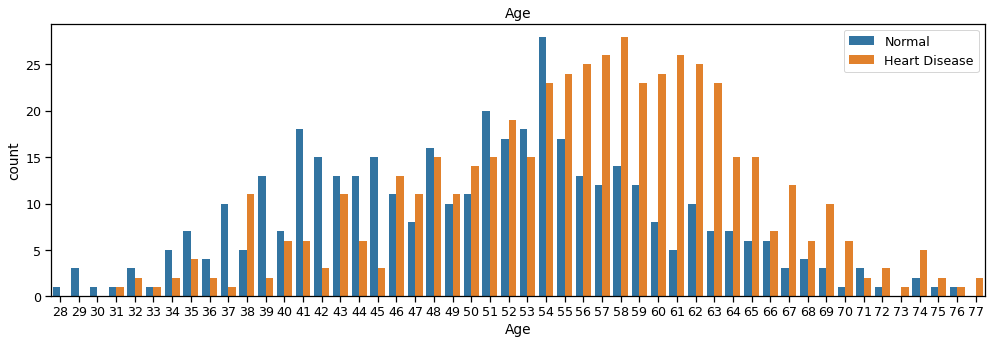
\includegraphics[scale=0.45]{age-count-chart.png}
	\caption{Age}
	\label{fig:age-count-chart}
\end{figure}
We can see that in \figurename~\ref{fig:age-count-chart} the occurrence of heart disease in the older ages from 55 to 77 is higher.

\begin{figure}[htb]
	\centering
	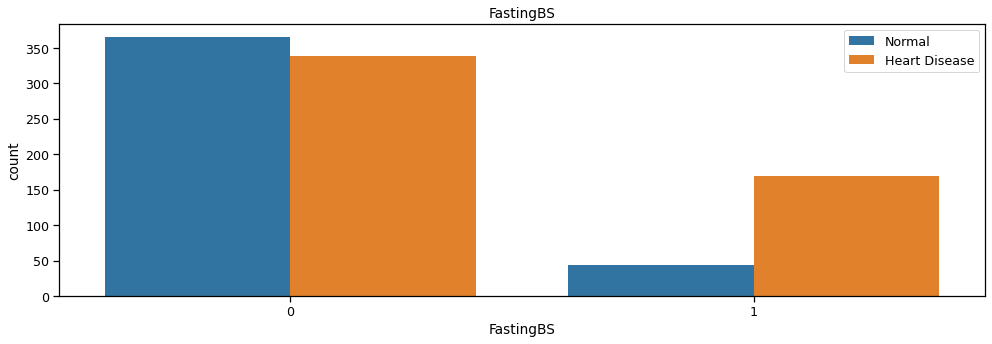
\includegraphics[scale=0.45,]{fasting-bs-chart.png}
	\caption{Fasting blood sugar}
	\label{fig:fasting-bs-chart}
\end{figure}

From the figure in ~\ref{fig:fasting-bs-chart} we can infer that higher fasting blood sugar is more likely to have heart disease.
\subsubsection{Plotting categorical values}

\begin{lstlisting}[language=Python, caption={Plotting categorical values}]
	# ploting categorical features with target
	for i in categorical:
		plt.figure(figsize=(10,5))
		sns.countplot(x=i, data=df, hue='HeartDisease', edgecolor='black')
		plt.legend(['Normal', 'Heart Disease'])
		plt.title(i)
		plt.show()
\end{lstlisting}

\begin{figure}[htb]
	\centering
	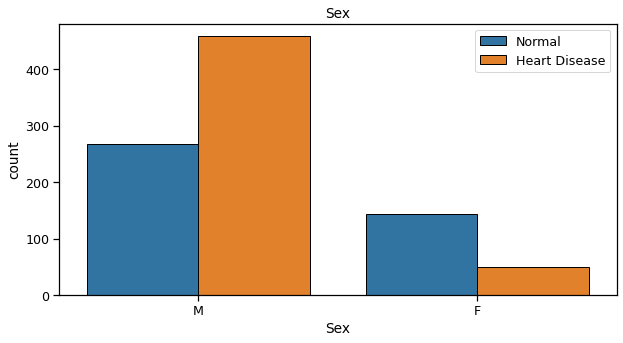
\includegraphics[scale=0.45]{sex-chart.png}
	\caption{Sex}
	\label{fig:sex-chart}
\end{figure}
\figurename~\ref{fig:sex-chart} shows that there's more occurrence of heart disease in males than females.

\begin{figure}[htb]
	\centering
	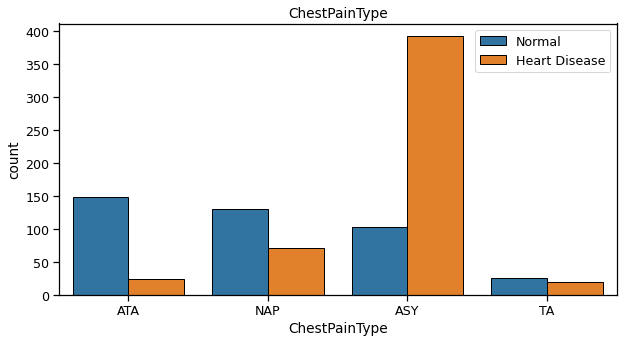
\includegraphics[scale=0.45]{chestpaintype-chart.png}
	\caption{Chest pain type}
	\label{fig:chestpaintype-chart}
\end{figure}
We can see from \figurename~\ref{fig:chestpaintype-chart} that the Asymptomatic chest pain type is highly correlated with heart disease.

\begin{figure}[htb]
	\centering
	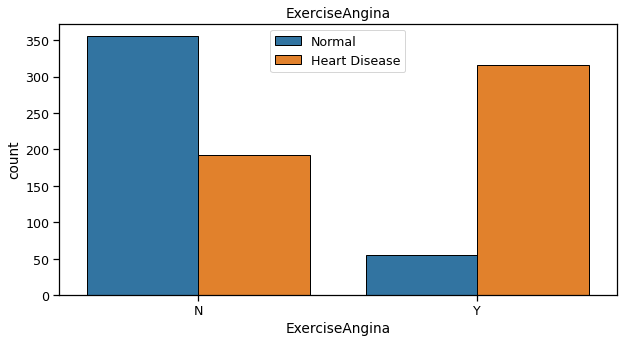
\includegraphics[scale=0.45]{exercise-angina-chart.png}
	\caption{Exercise angina}
	\label{fig:exercise-angina-chart}
\end{figure}

\begin{figure}[htb]
	\centering
	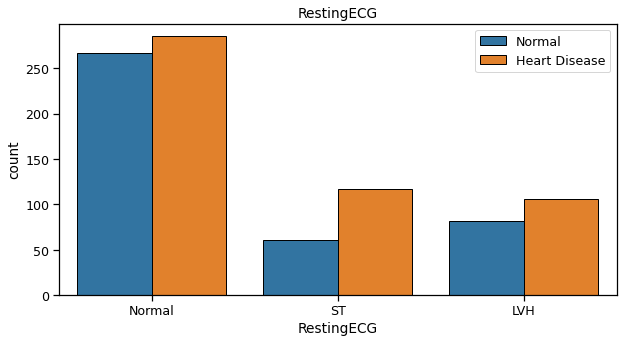
\includegraphics[scale=0.45]{restingecg-chart.png}
	\caption{Resting electrocardiogram results}
	\label{fig:restingect-chart}
\end{figure}

\subsection{Data preprocessing}
The preprocessing steps in the following subsections were applied on the dataset.
\subsubsection{Imputation}
Before imputation, we have to check for missing values in the dataset.
\begin{lstlisting}[language=Python, caption=Dataset information]
	df.info()\end{lstlisting}
Output:
\begin{lstlisting}[numbers=none]
	RangeIndex: 918 entries, 0 to 917
	Data columns (total 12 columns):
	#   Column          Non-Null Count  Dtype  
	---  ------          --------------  -----  
	0   Age             918 non-null    int64  
	1   Sex             918 non-null    object 
	2   ChestPainType   918 non-null    object 
	3   RestingBP       918 non-null    int64  
	4   Cholesterol     918 non-null    int64  
	5   FastingBS       918 non-null    int64  
	6   RestingECG      918 non-null    object 
	7   MaxHR           918 non-null    int64  
	8   ExerciseAngina  918 non-null    object 
	9   Oldpeak         918 non-null    float64
	10  ST_Slope        918 non-null    object 
	11  HeartDisease    918 non-null    int64  
	dtypes: float64(1), int64(6), object(5)
	memory usage: 86.2+ KB
\end{lstlisting}

\comment{

We can see from the output that there are no null values in the dataset. Also, The \textit{string} columns in the dataset are represented as \textit{object} and need to be converted to \textit{string} types.


\begin{lstlisting}[language=Python, caption={Convert object columns to string}]
	string_col = df.select_dtypes(include="object").columns
	df[string_col]=df[string_col].astype("string")
\end{lstlisting}
}

\subsubsection{Feature scaling}
Feature scaling was done using the MinMaxScaler class in the sklearn library on the dataframe used to train non-tree based algorithms.

\begin{lstlisting}[language=Python, caption={Scaling with MinMaxScaler}]
	from sklearn.preprocessing import MinMaxScaler
	
	scal = MinMaxScaler()
	X_train = scal.fit_transform(df_nontree[feature_col_nontree].values)
	Y_train = df_nontree[target_col]
	df[string_col]=df[string_col].astype("string")
\end{lstlisting}

\subsubsection{Handling of categorical values}
Label encoding is used in this study to encoding is used for Decision tree model while One-Hot encoder is used for the non-tree based algorithms.

\begin{lstlisting}[language=Python, caption={Applying Label Encoder to the dataframe}]
	from sklearn.preprocessing import LabelEncoder
	
	le = LabelEncoder()
	df_cat = df[string_col].apply(le.fit_transform)
\end{lstlisting}

\begin{lstlisting}[language=Python, caption={Applying One-Hot Encoder to the dataframe}]
	from sklearn.preprocessing import OneHotEncoder
	from sklearn.compose import make_column_transformer
	
	target_col="HeartDisease"
	
	
	df_nontree = df.drop(target_col,axis=1)
	
	ohe = OneHotEncoder(handle_unknown='ignore')
	
	transformer = make_column_transformer(
		(OneHotEncoder(), string_col),
		remainder='passthrough',
		verbose_feature_names_out=False
	)
	
	transformed = transformer.fit_transform(df_nontree)
		df_nontree = pd.DataFrame(
		transformed, 
		columns=transformer.get_feature_names_out()
	)
\end{lstlisting}

\subsection{Training and Performance analysis}
The dataset was split using StratifiedKFold over 5 folds for cross validation and the accuracy of every fold was calculated using area under the ROC curve (AUC) to get precision, recall and f1-score.


\subsubsection{Logistic Regression}
Logistic regression had a peak accuracy of 88\% after cross-validation

\subsubsection{Naive Bayes}
Naive Bayes had a peak accuracy of 88.3\% after cross-validation

\subsubsection{KNN}
K-nearest neighbours had a peak accuracy of 91.6\% after cross-validation

\subsubsection{Decision Tree}
Decision Tree had a peak accuracy of 77.2\% after cross-validation

\section{Web Server module}
The web server contains the views and the inference engine. The views module is responsible for responding to http request from a client. The home page displays a form \figurename~\ref{fig:site-2} for the user to enter the medical data. When the data form is sent, the server processes the data and returns the results and inference in the result page, \figurename~\ref{fig:site-3}

\begin{lstlisting}[language=Python, caption={app.py}, label={lst:app.py}]
	from flask import Flask
	from flask_assets import Bundle, Environment
	from app.views.index import index
	from app.config import Config
	
	def create_app():
		app = Flask(__name__)
		app.config.from_object(Config)
		assets = Environment(app)
		
		css = Bundle("src/main.css", output="dist/main.css")
		
		assets.register("css", css)
		css.build()
		
		app.register_blueprint(index)
		
		return app
\end{lstlisting}

\begin{figure}[htb]
	\centering
	\makebox[0cm]{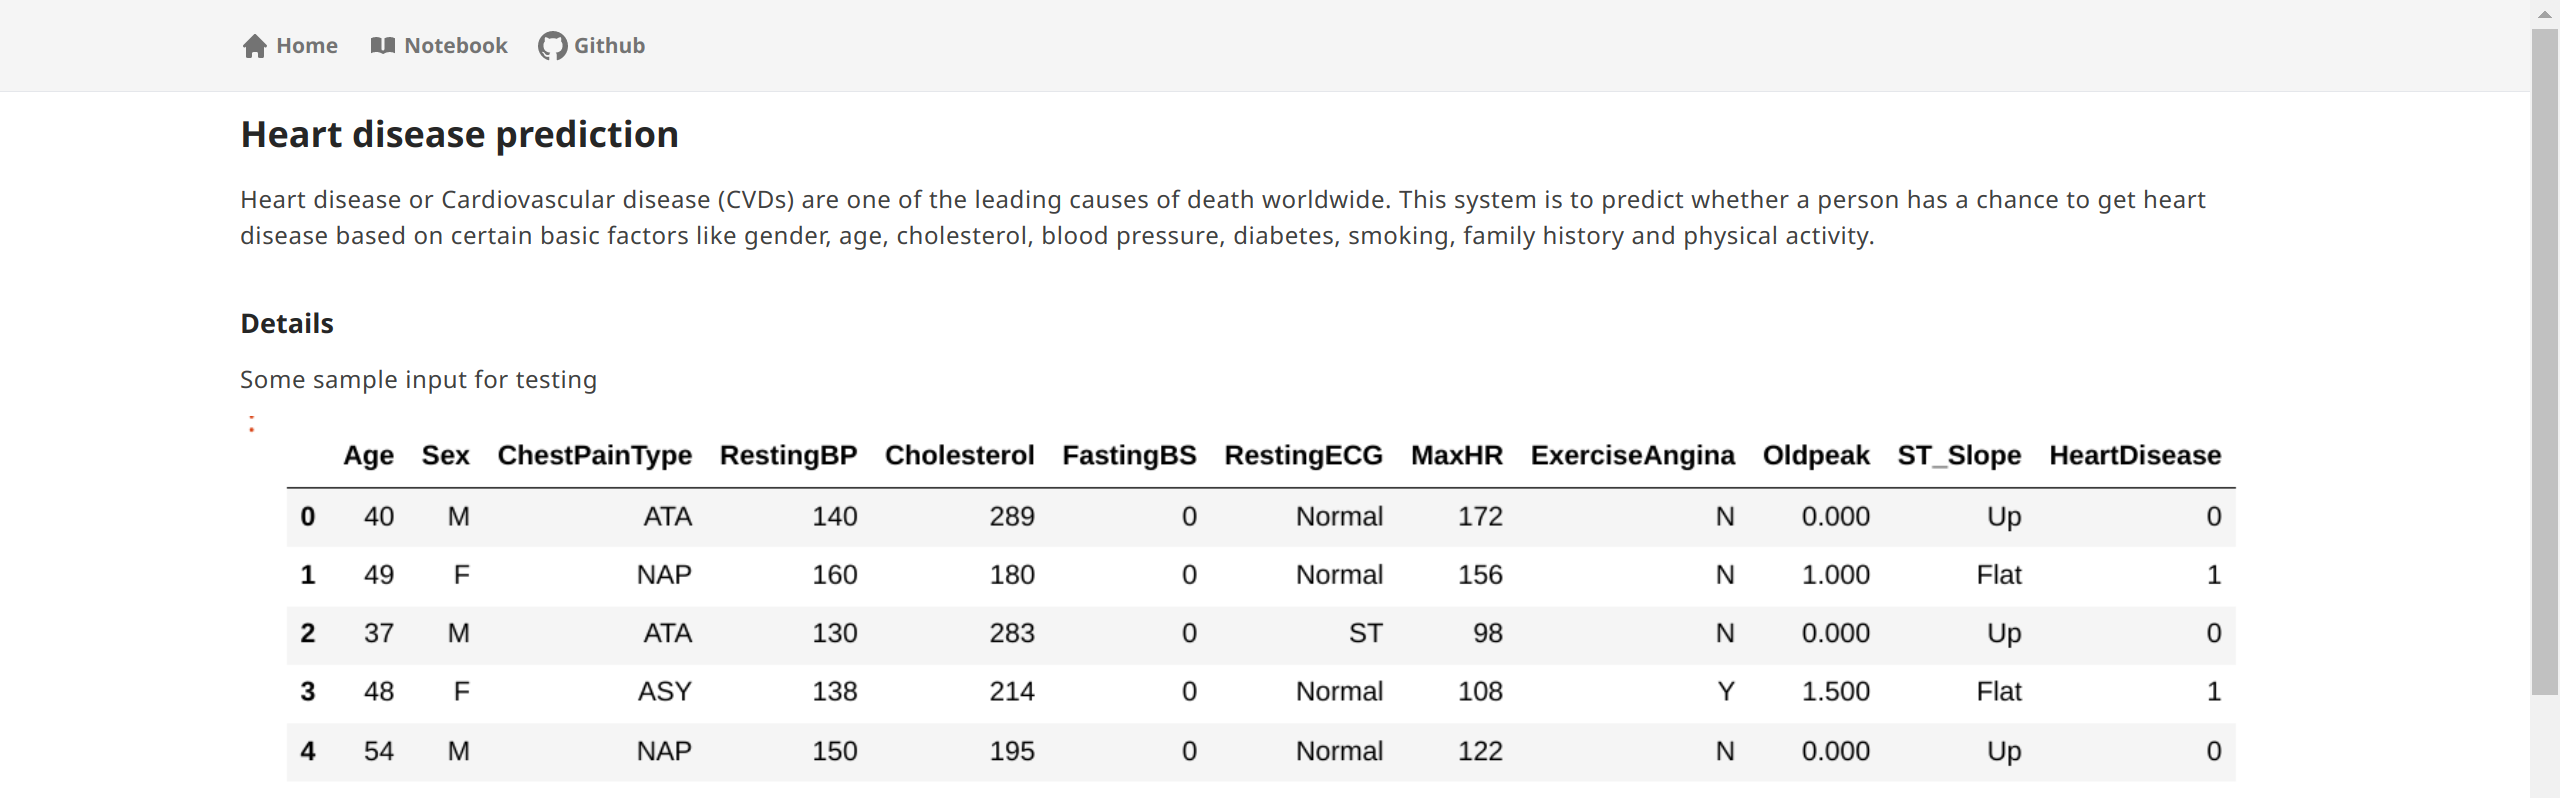
\includegraphics[scale=0.5]{site-1.png}}
	\caption{Webpage top}
	\label{fig:site-1}
\end{figure}

\begin{figure}[htb]
	\centering
	\makebox[0cm]{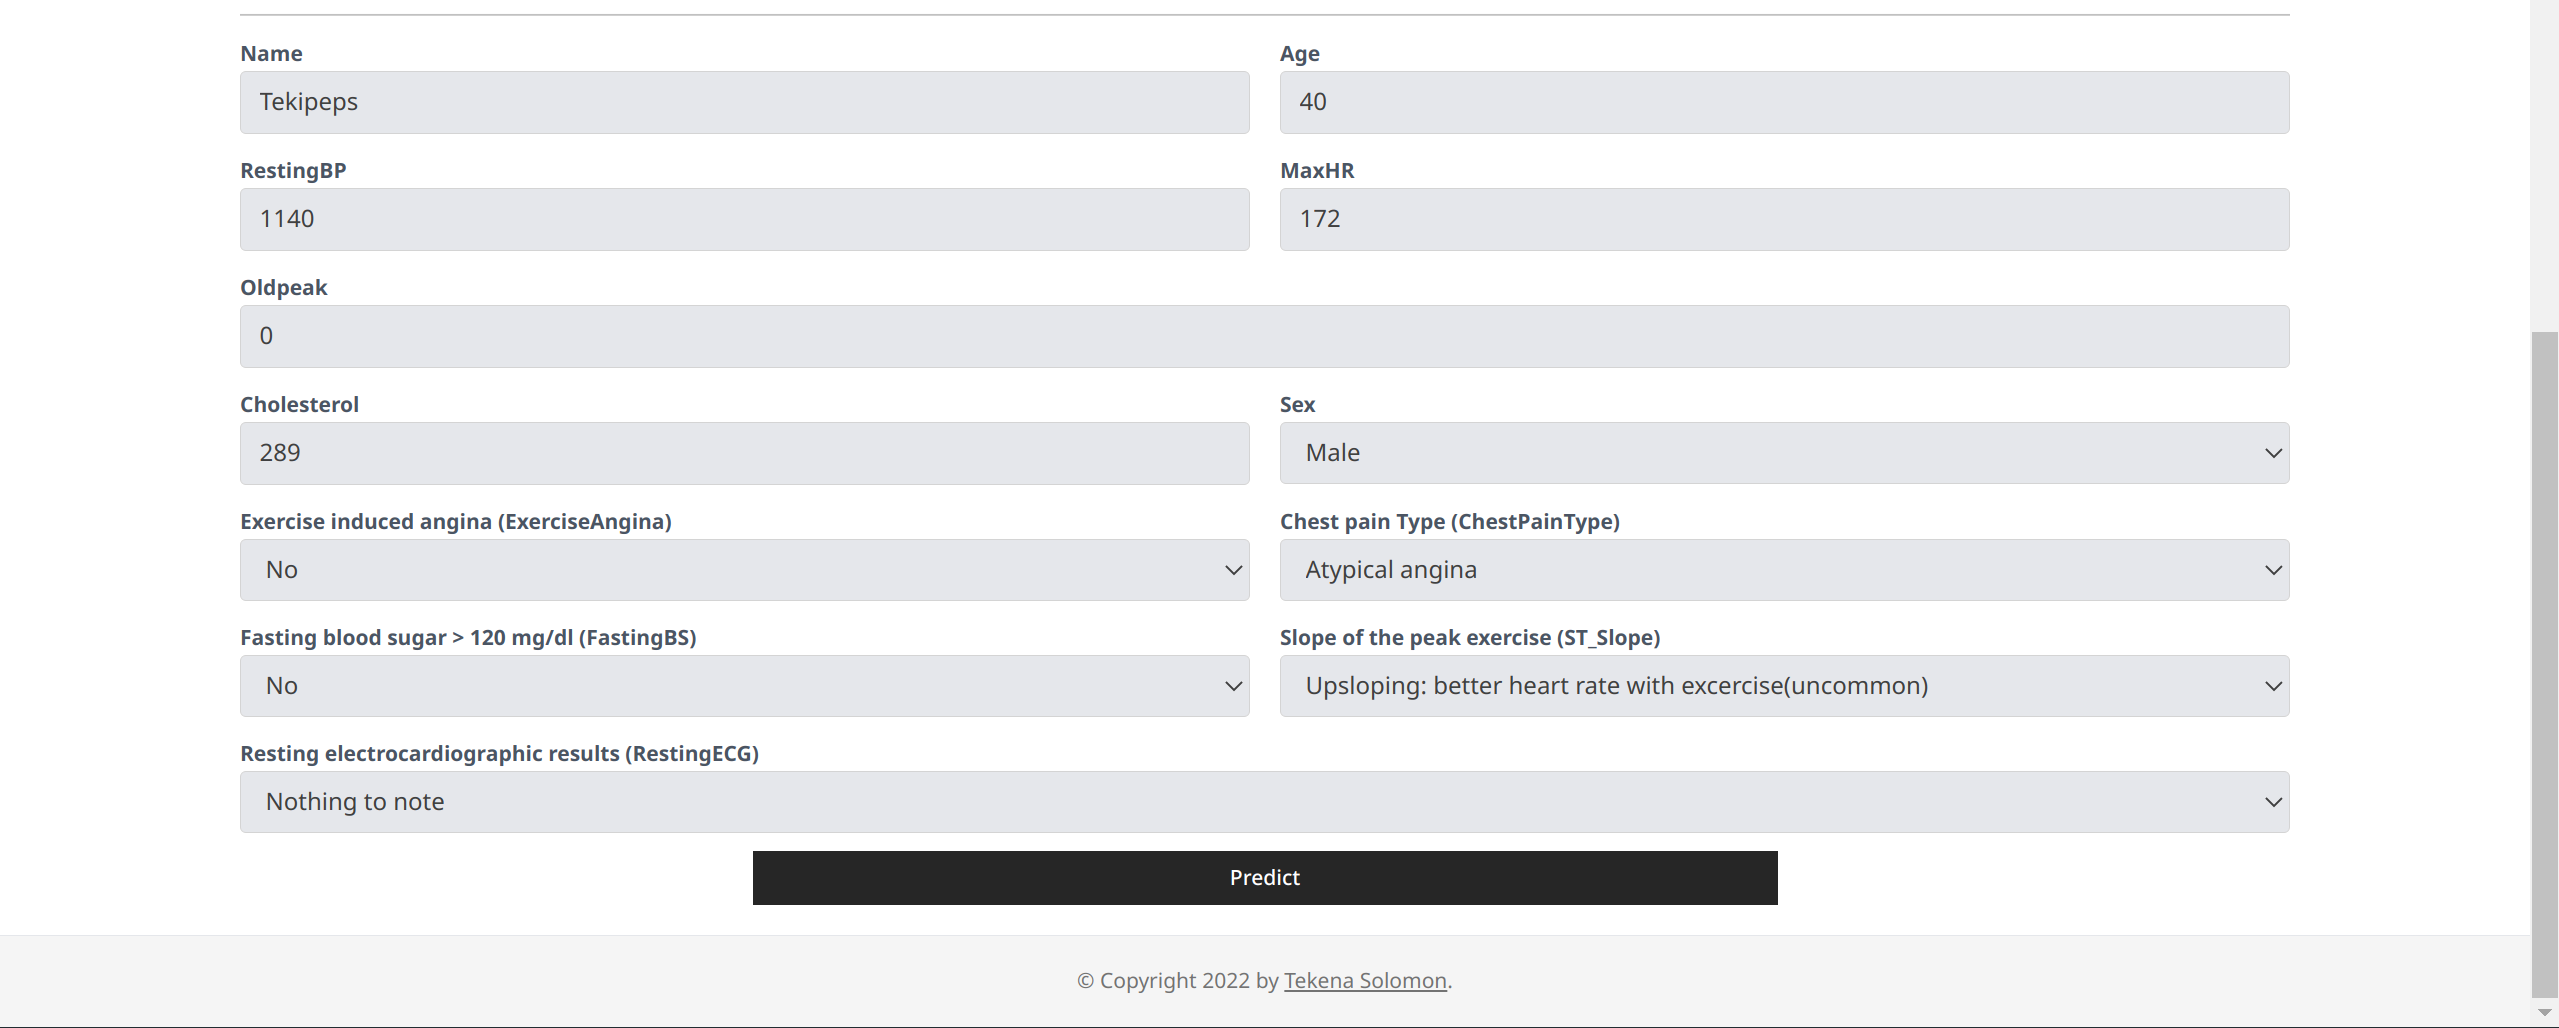
\includegraphics[scale=0.5]{site-2.png}}
	\caption{Webpage form}
	\label{fig:site-2}
\end{figure}
\begin{figure}[htb]
	\centering
	\makebox[0cm]{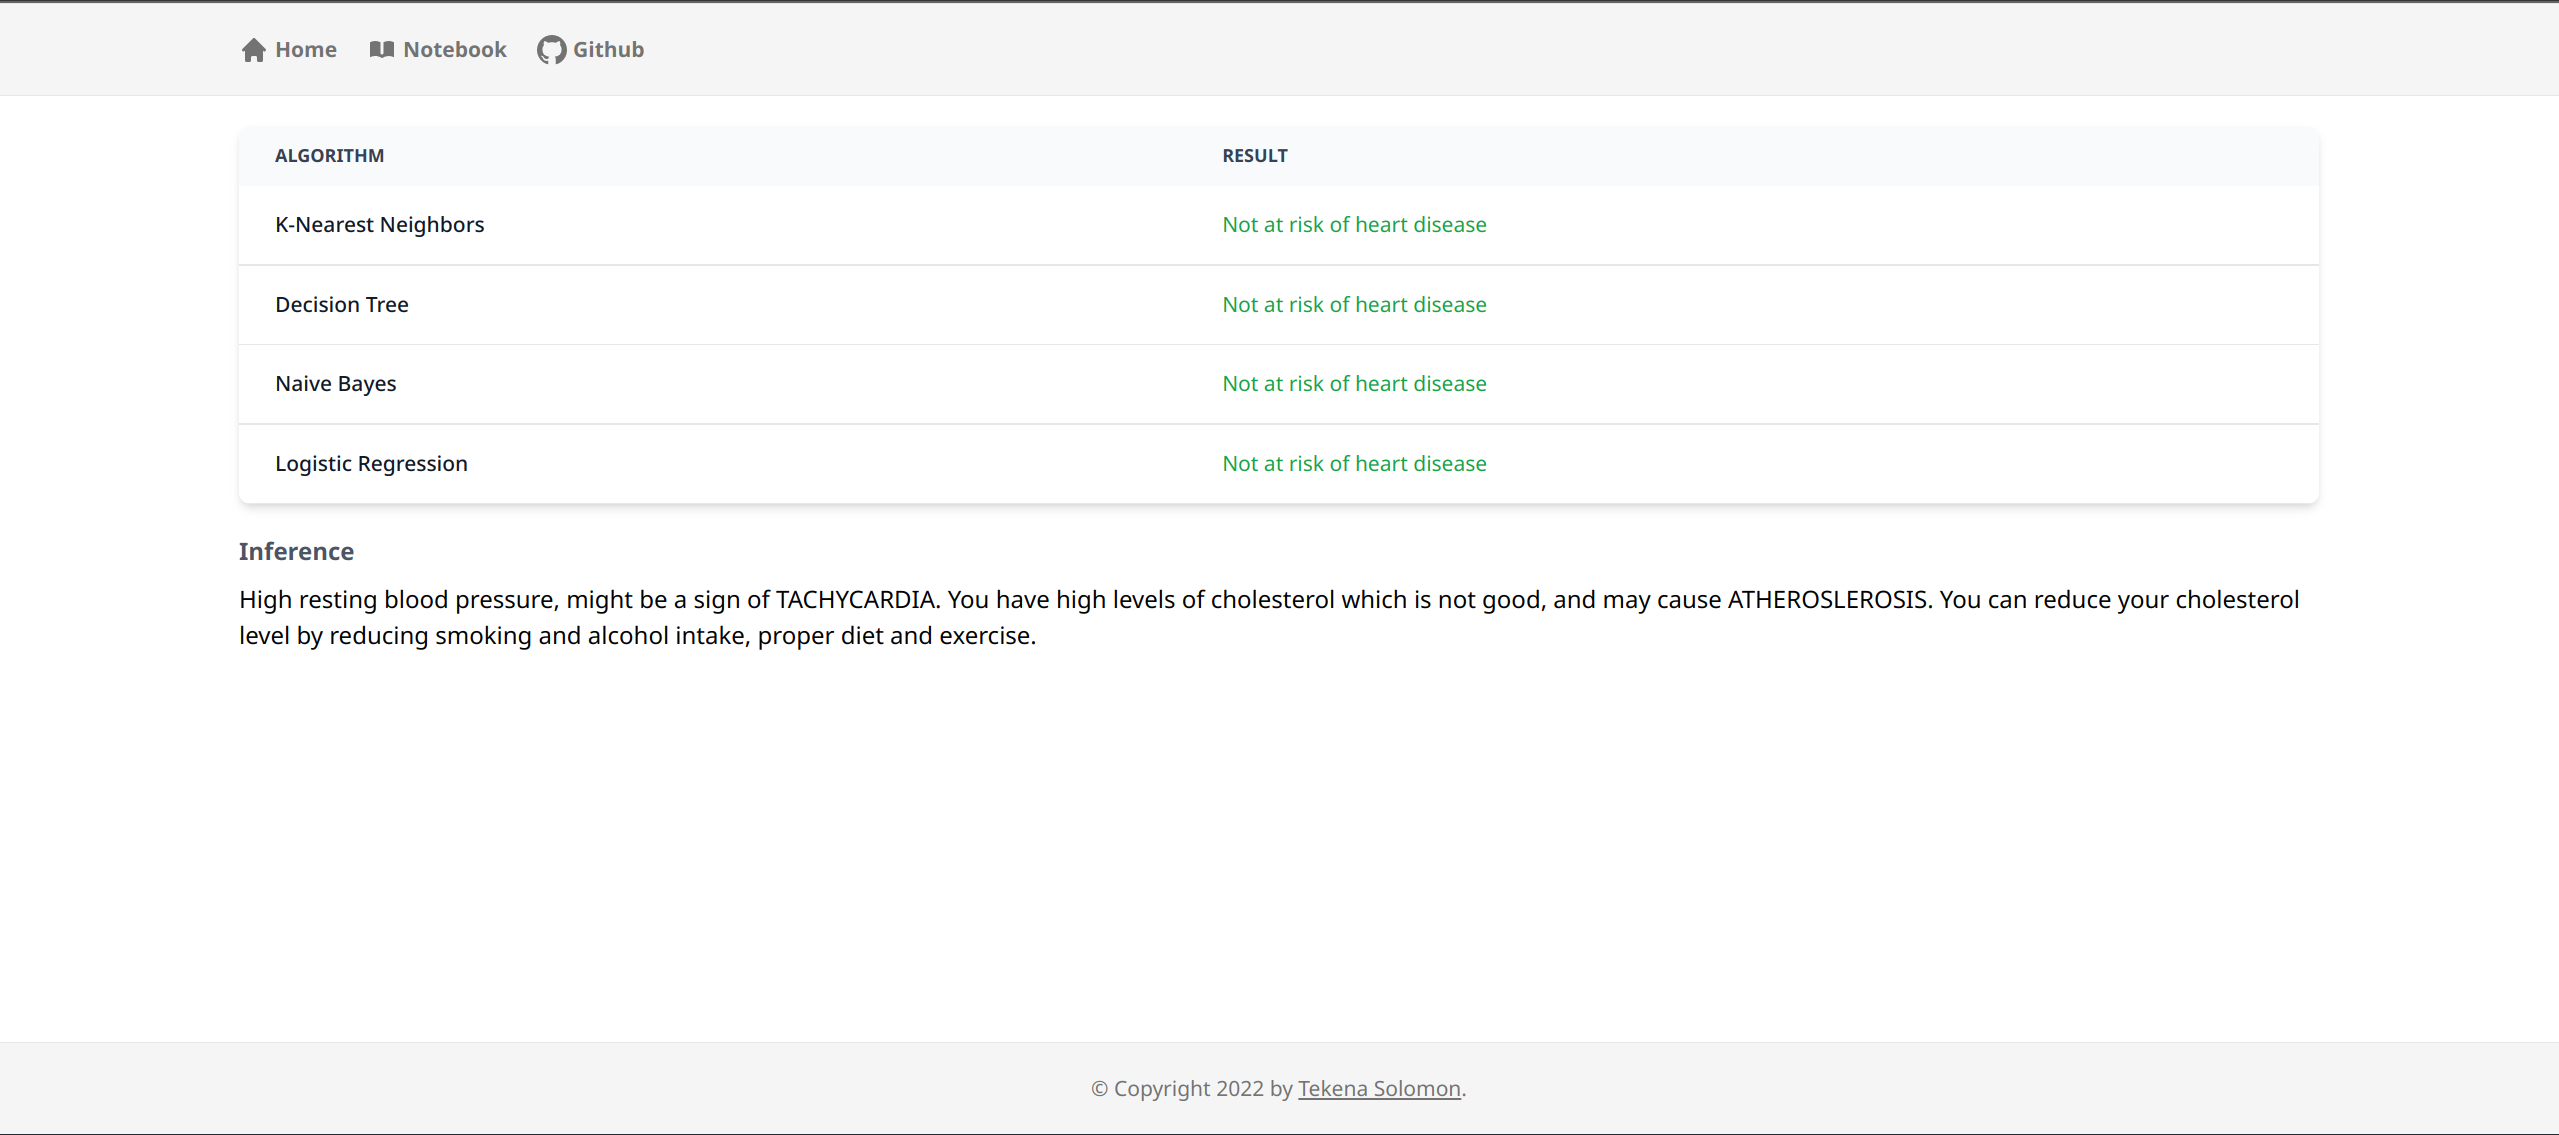
\includegraphics[scale=0.5]{site-3.png}}
	\caption{Results page}
	\label{fig:site-3}
\end{figure}



\section{Inference engine module}
The inference engine module is responsible for producing inference on the medical data. It consists of the knowledge base and the parser.

\subsection{Knowledge base}
The knowledge base is encoded in yaml format. It contains the attributes and conditions (rules) on those attributes that produce an inference.

\begin{figure}[htb]
	\centering
	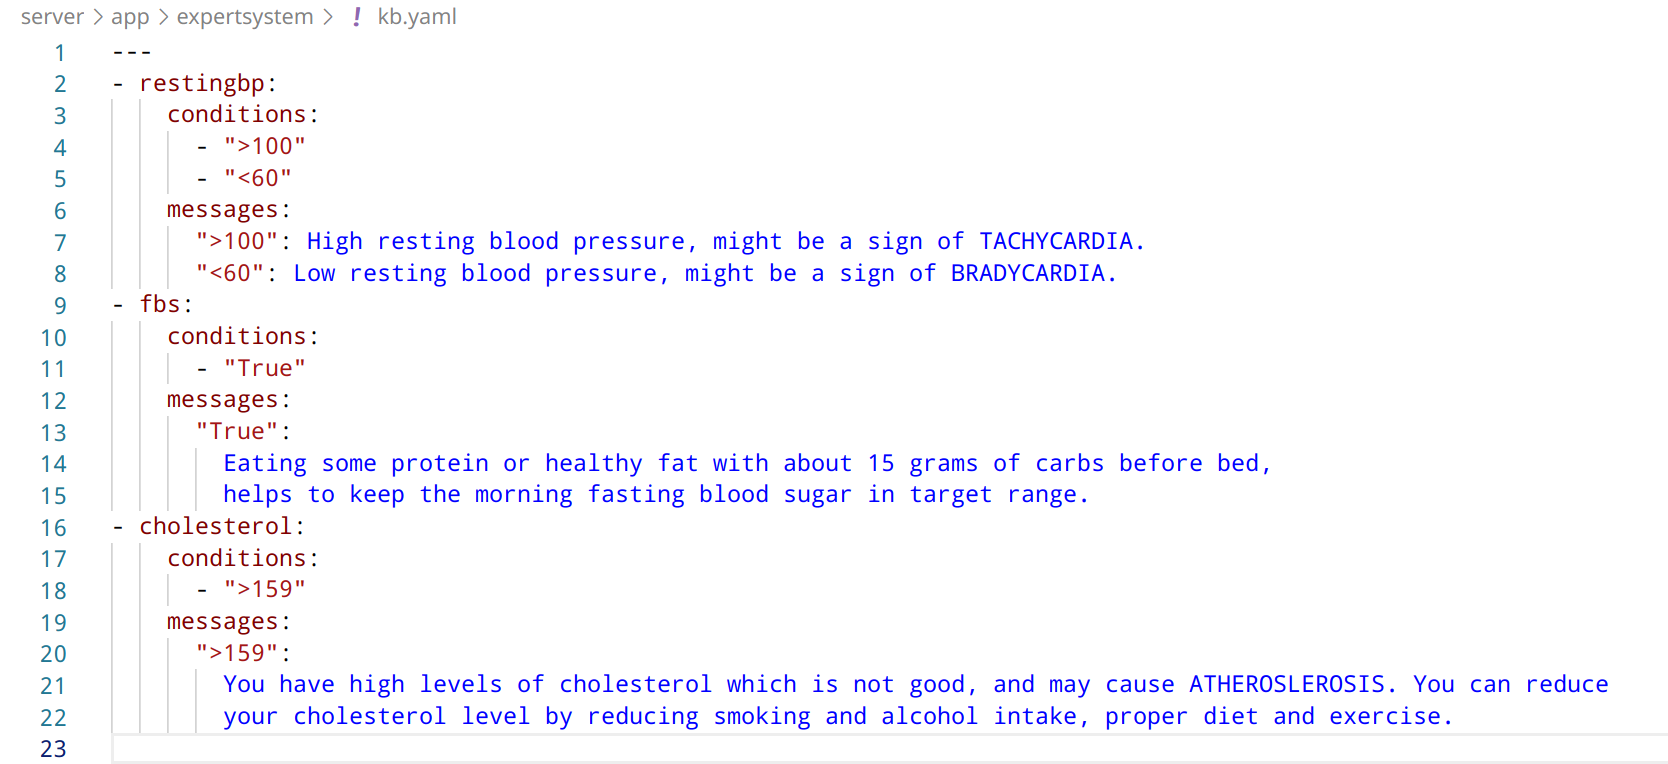
\includegraphics[scale=0.67]{kb.png}
	\caption{Knowledge base}
	\label{fig:kb}
\end{figure}

\subsection{Parser}
The parser parses the knowledge base and provides output based on the medical data. The parser takes the medical data as a lookup table to be able to call the values while parsing.

\begin{lstlisting}[language=Python, caption={Knowledge base parser}, numbers=none]
	def parse_conditions(kb, table):
		inference = ""
		for attribute in kb:
			attrname = list(attribute.keys())[0]
			for condition in attribute[attrname]["conditions"]:
				if condition.startswith(">"):
					val = int(condition[1:])
					if table[attrname] > val:
						inference += attribute[attrname]["messages"][condition] + " "
				elif condition.startswith("<"):
					val = int(condition[1:])
					if table[attrname] < val:
						inference += attribute[attrname]["messages"][condition] + " "
				elif condition == "True":
					if table[attrname] == True:
						inference += attribute[attrname]["messages"][condition] + " "
				elif condition == "False":
					if table[attrname] == False:
						inference += attribute[attrname]["messages"][condition] + " "
		
		return inference
	
\end{lstlisting}

\comment{summary, conclusion and recommendation}
\chapter{Conclusion}
\noindent
This chapter is the last part of the study. It is split into 3 parts: section 5.1 gives a summary of the whole study, section 5.2 gives the conclusion based on the project, and section 5.3 gives suggestions for future study.

\section{Summary}
Heart disease analysis are the most difficult clinical challenges. It is dependent on a thorough examination of the patient's clinical data by clinical specialists. Because of advancements in AI and IT, clinical specialists are eager to create a profoundly accurate, productive, and strong predictive model for heart disease. Data analysis and machine (AI) methodologies were used to assess and summarize the risk of getting heart disease. Expert system technology is also implemented to provide a description of how the patient can improve their heart health based on encoded expert knowledge.

\section{Conclusion}
From this study, I was able to attain my research goals. Heart disease datasets from the Machine Learning Repository have been looked at, cleaned up, and preprocessed to get them ready for the classification process. It has been shown to be a very useful method for auto-tuning parameters and choosing the best set of features that affect the chances of having heart disease. Humans can't be replaced by computers, but by comparing the results of computer-aided diagnosis with pathological findings, doctors can learn more about how to evaluate the areas that computer-aided diagnosis highlights.

\section{Recommendation}
Medical diagnosis is seen as an important but difficult task that needs to be done correctly and efficiently. It would be incredibly advantageous to automate this process. Clinical decisions are often made by doctors based on their gut feelings and years of experience, not on the information-rich data that is hidden in the database. This practice causes biases, mistakes, and high medical costs, all of which hurt the quality of care given to patients. Data mining has the potential to create an environment that is full of knowledge and can help make clinical decisions that are much better.





\comment {
Definition. An appendix contains supplementary material that is not an essential part of the text itself but which may be helpful in providing a more comprehensive understanding of the research problem or it is information that is too cumbersome to be included in the body of the paper.}

\renewcommand{\bibname}{References}
\bibliographystyle{apalike}
\bibliography{chapters/references}

\appendix
\chapter{Appendix Title}
\chapter{Listings}

\begin{lstlisting}[language=Python, caption={Correlation chart}, label={lst:corr}]
	pd.options.display.float_format = "{:,.3f}".format
	plt.figure(figsize=(10,8))
	sns.set_context('notebook',font_scale = 1.15)
	sns.heatmap(df.corr(),annot=True, linewidths=1)
	plt.savefig("corr.png")
	plt.show()
\end{lstlisting}

\begin{lstlisting}[language=Python, caption={Plotting select numerical features with target column}, label={lst:plot-numerical}]
	cols_to_plot = ["Age", "FastingBS"]
	for i in cols_to_plot:
	plt.figure(figsize=(14,5))
	sns.countplot(x=df[i], data=df, hue='HeartDisease')
	plt.legend(['Normal', 'Heart Disease'])
	plt.title(i)
	plt.tight_layout()
\end{lstlisting}

\begin{lstlisting}[language=Python, caption={Plotting categorical values}, label={lst:plot-categorical}]
	# ploting categorical features with target
	for i in categorical:
	plt.figure(figsize=(10,5))
	sns.countplot(x=i, data=df, hue='HeartDisease', edgecolor='black')
	plt.legend(['Normal', 'Heart Disease'])
	plt.title(i)
	plt.show()
\end{lstlisting}

\begin{lstlisting}[numbers=none, label={lst:dataset-info-output}, caption={Dataset information}]
	RangeIndex: 918 entries, 0 to 917
	Data columns (total 12 columns):
	#   Column          Non-Null Count  Dtype  
	---  ------          --------------  -----  
	0   Age             918 non-null    int64  
	1   Sex             918 non-null    object 
	2   ChestPainType   918 non-null    object 
	3   RestingBP       918 non-null    int64  
	4   Cholesterol     918 non-null    int64  
	5   FastingBS       918 non-null    int64  
	6   RestingECG      918 non-null    object 
	7   MaxHR           918 non-null    int64  
	8   ExerciseAngina  918 non-null    object 
	9   Oldpeak         918 non-null    float64
	10  ST_Slope        918 non-null    object 
	11  HeartDisease    918 non-null    int64  
	dtypes: float64(1), int64(6), object(5)
	memory usage: 86.2+ KB
\end{lstlisting}

\begin{lstlisting}[language=Python, caption={Scaling with MinMaxScaler}, label={lst:min-max-scaler}]
	from sklearn.preprocessing import MinMaxScaler
	
	scal = MinMaxScaler()
	X_train = scal.fit_transform(df_nontree[feature_col_nontree].values)
	Y_train = df_nontree[target_col]
	df[string_col]=df[string_col].astype("string")
\end{lstlisting}

\begin{lstlisting}[language=Python, caption={Applying Label Encoder to the dataframe}, label={lst:label-encoding}]
	from sklearn.preprocessing import LabelEncoder
	
	le = LabelEncoder()
	df_cat = df[string_col].apply(le.fit_transform)
\end{lstlisting}
\begin{lstlisting}[language=Python, caption={Applying One-Hot Encoder to the dataframe}, label={lst:one-hot-encoding}]
	from sklearn.preprocessing import OneHotEncoder
	from sklearn.compose import make_column_transformer
	target_col="HeartDisease"
	df_nontree = df.drop(target_col,axis=1)	
	ohe = OneHotEncoder(handle_unknown='ignore')
	transformer = make_column_transformer(
		(OneHotEncoder(), string_col),
			remainder='passthrough',
			verbose_feature_names_out=False
		)
		
	transformed = transformer.fit_transform(df_nontree)
	df_nontree = pd.DataFrame(
		transformed, 
		columns=transformer.get_feature_names_out()
	)
\end{lstlisting}

\begin{lstlisting}[language=Python, caption={App Entrypoint}, label={lst:web-server-entrypoint}]
	from flask import Flask
	from flask_assets import Bundle, Environment
	from app.views.index import index
	from app.config import Config
	
	def create_app():
	app = Flask(__name__)
	app.config.from_object(Config)
	assets = Environment(app)
	
	css = Bundle("src/main.css", output="dist/main.css")
	
	assets.register("css", css)
	css.build()
	
	app.register_blueprint(index)
	
	return app
\end{lstlisting}

\begin{lstlisting}[language=Python, caption={Knowledge base parser}, label={lst:kb-parser}]
	def parse_conditions(kb, table):
		inference = ""
		for attribute in kb:
			attrname = list(attribute.keys())[0]
			for condition in attribute[attrname]["conditions"]:
				if condition.startswith(">"):
					val = int(condition[1:])
					if table[attrname] > val:
						inference += attribute[attrname]["messages"][condition] + " "
				elif condition.startswith("<"):
					val = int(condition[1:])
					if table[attrname] < val:
						inference += attribute[attrname]["messages"][condition] + " "
				elif condition == "True":
					if table[attrname] == True:
						inference += attribute[attrname]["messages"][condition] + " "
				elif condition == "False":
					if table[attrname] == False:
						inference += attribute[attrname]["messages"][condition] + " "
		return inference
\end{lstlisting}

\end{document}